\section{Mobiscope Platform}
\label{sec:platform}

This section describes the goals for our monitoring approach, and how \platname achieves these goals using proxying.
We show that our approach imposes reasonable overheads, and we describe how our IRB-approved study protects user privacy.

\subsection{Goals}
\label{sec:goals}
Our primary goal is \emph{to monitor all the Internet traffic from mobile devices regardless of the operating system, wireless access technology, and the ISPs used by the mobile device}.
To achieve this goal, we identify the following desirable properties for a measurement platform:
\begin{packedenumerate}
\item \emph{Portable.} Our approach should work on all major device OSes without requiring support from carriers or ISPs.
\item \emph{Pervasive.} We should be able to measure traffic regardless of the location, access technology, and ISPs used by mobile devices.
\item \emph{Passive.} We wish to understand the network traffic naturally generated by users and their devices, requiring passive monitoring.
\item \emph{Deployable.} We want a low barrier to entry to facilitate large-scale adoption with minimal impact on the user experience. \tbd{We need to say easy to controlled perform experiments}
\end{packedenumerate}

\subsection{Approach}

We now describe how we achieve these goals using proxying. 
Specifically, we use two approaches to proxy mobile traffic: secure proxying via virtual private networks (VPNs) and insecure transparent proxying. 
These two approaches allow us to measure traffic with and without carrier interposition, respectively. 

\subsubsection{VPN Proxying}
\label{sec:platform-vpn}

VPN tunnels over Wi-Fi and the cellular interface are supported by Android, BlackBerry, Bada, and iOS. 
Mobile OSes support VPNs primarily to satisfy their enterprise clients that use VPNs to securely connect to their enterprise networks. 
We use VPNs to proxy Internet traffic and monitor the mobile Internet traffic that flows through our VPN proxy.  

All our goals can be achieved if we ensure that mobile devices use our VPN proxy to their Internet traffic.
The use of VPNs by enterprise clients meets our goals of portability, passiveness, and deployability.
To meet our goal of pervasiveness we must ensure that all the Internet traffic is tunneled through our VPN proxy. 
Currently, all iOS devices (version 3.0 and above) support a feature called ``VPN On-Demand''. 
\emph{VPN On-Demand} forces the iOS device to use VPN tunnels when connecting to a specified set of domains.
Using trial-and-error, we discovered that VPN On-Demand uses suffix matching to determine which domains require a VPN connection.
We use this knowledge to configure \emph{VPN On-Demand} such that iOS devices use a VPN tunnel to access the Internet.
Android version 4.2 and above support ``Always On'' VPN connections that are established regardless of the destination for network traffic. 
Furthermore, Android version 4.0 and above provide an API that allows applications to manage VPN tunnels. 
These APIs are used by open source android applications and we extend one such application to support ``Always On'' VPN connections. We are therefore able to ensure pervasive monitoring of iOS and Android devices. 

The use IPsec by mobile devices for pervasive VPN tunnels limited our choice of VPN daemons to manage VPN tunnels on our proxying server.
Though VPN daemons manage tunnels created using protocols such as PPTP and L2TP, the ``VPN On-Demand'' feature of iOS is available only for VPN tunnels that use IPsec.  
To the best of our knowledge, the only publicly available VPN daemon that uses IPsec in Linux \emph{without any kernel modifications} is Strongswan~\cite{strongswan}.
Strongswan also supports the faster IKEv2~\cite{rfc5996} based authentication which is supported by Android devices. 

The IPsec implementation in the Linux kernel is not suitable to traffic monitoring when the server running the VPN daemon is used to proxy Internet traffic. 
A VPN Proxy, apart from serving VPN tunnels, relies on NAT to proxy Internet traffic. 
When a mobile device establishes a VPN tunnel, the VPN server assigns it assigned a private IP address. 
The mobile device therefore has two IP addresses, a private address assigned by the VPN server, and a public IP address assigned by the service provider. 
The public IP address is used only to communicate with the VPN server while all other communication uses the private IP address. 
Therefore all the traffic that would have used the public IP address when the VPN tunnel was not present, now uses the private IP address.  
These packets that use the private IP are encapsulated and encrypted using IPsec and sent to the VPN server. 
The VPN server decapsulates these packets before forwarding them. 
Before forwarding the packet, the VPN server must perform NAT because these private IP address cannot used in the Internet. 
The use of NAT and IPsec implies that the forwarding each packet by the server is governed by two rules: one rule to enforce IPsec encryption and decryption of packets that contain the public IP of the mobile device, and the other that enforces NAT for packets with the private IP address. 

\begin{figure}
\begin{center}
\subfloat[Packet from mobile device. \emph{Tcpdump can capture packets at step (2)~d~$\rightarrow$~m, (4)~v~$\rightarrow$~w, and (7)~m~$\rightarrow$~w.}]{\label{fig:packet-monitor-a}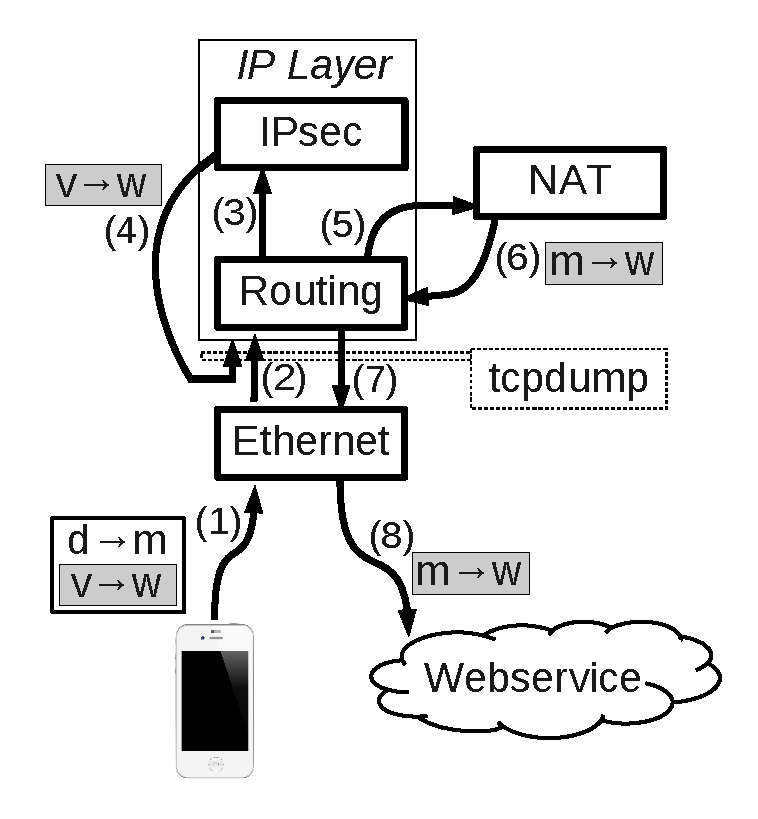
\includegraphics[width=0.47\columnwidth]{figures/packet-monitoring-a.pdf}}
\hspace{0.05\columnwidth}
\subfloat[Packet to mobile device. \emph{Tcpdump can capture packets at step (2)~w~$\rightarrow$~m and (7)~m~$\rightarrow$~d, however it is cannot log the packet w~$\rightarrow$~v.}]{\label{fig:packet-monitor-b}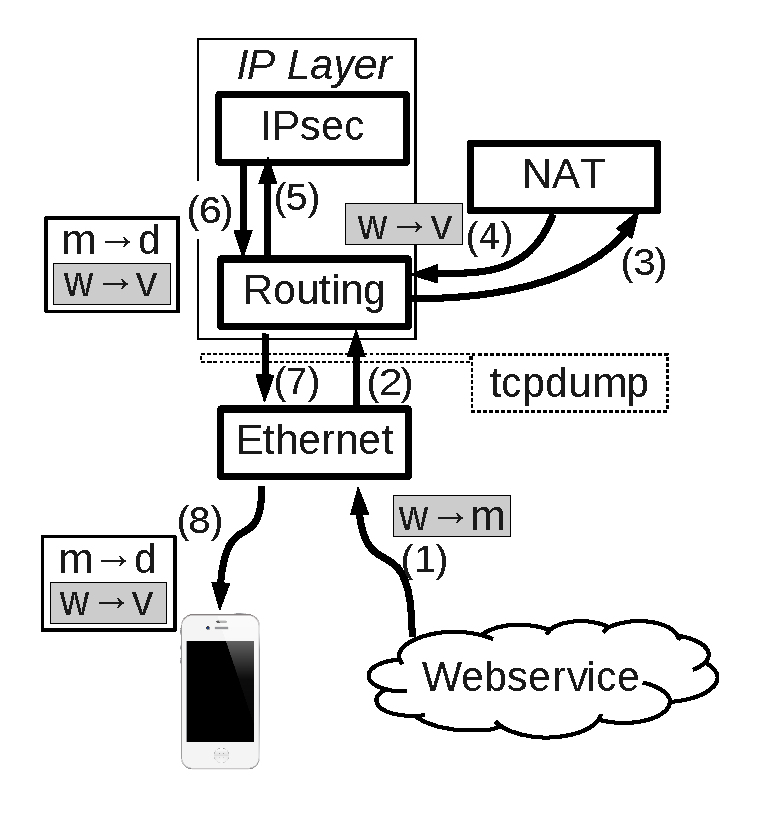
\includegraphics[width=0.47\columnwidth]{figures/packet-monitoring-b.pdf}}
\newline
\subfloat[Packet from mobile device. \emph{Tcpdump monitoring packets on the tun device can capture packets at step (5)~v~$\rightarrow$~w, and (6)~v'~$\rightarrow$~w.}]{\label{fig:packet-monitor-c}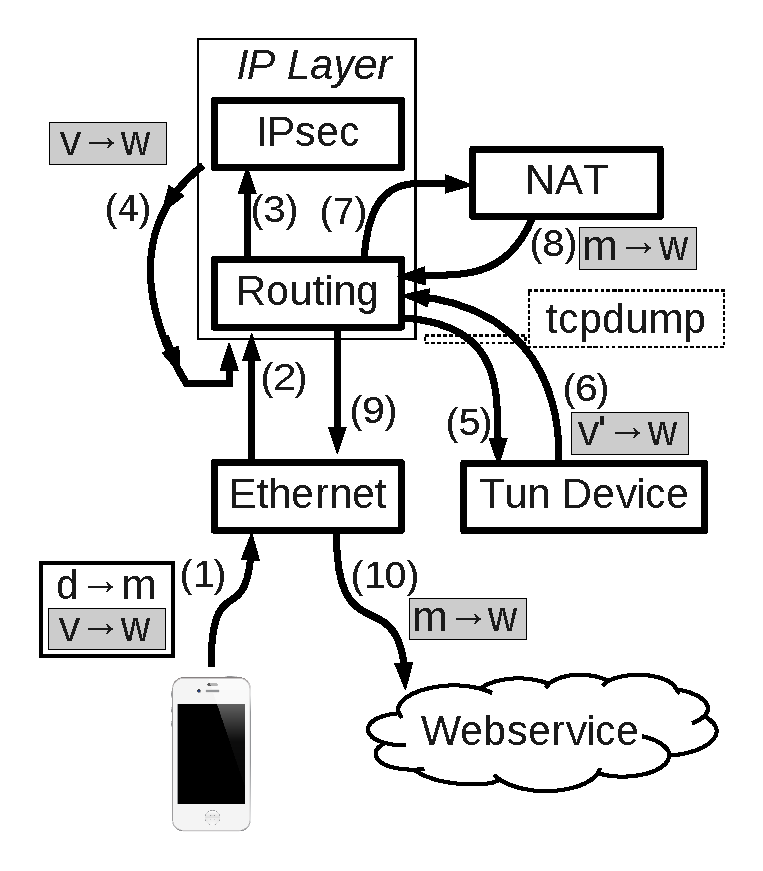
\includegraphics[width=0.47\columnwidth]{figures/packet-monitoring-c.pdf}}
\hspace{0.05\columnwidth}
\subfloat[Packet to mobile device. \emph{Tcpdump monitoring packets on the tun device can capture packets at step (5)~w~$\rightarrow$~v', and (6)~w~$\rightarrow$~v.}]{\label{fig:packet-monitor-d}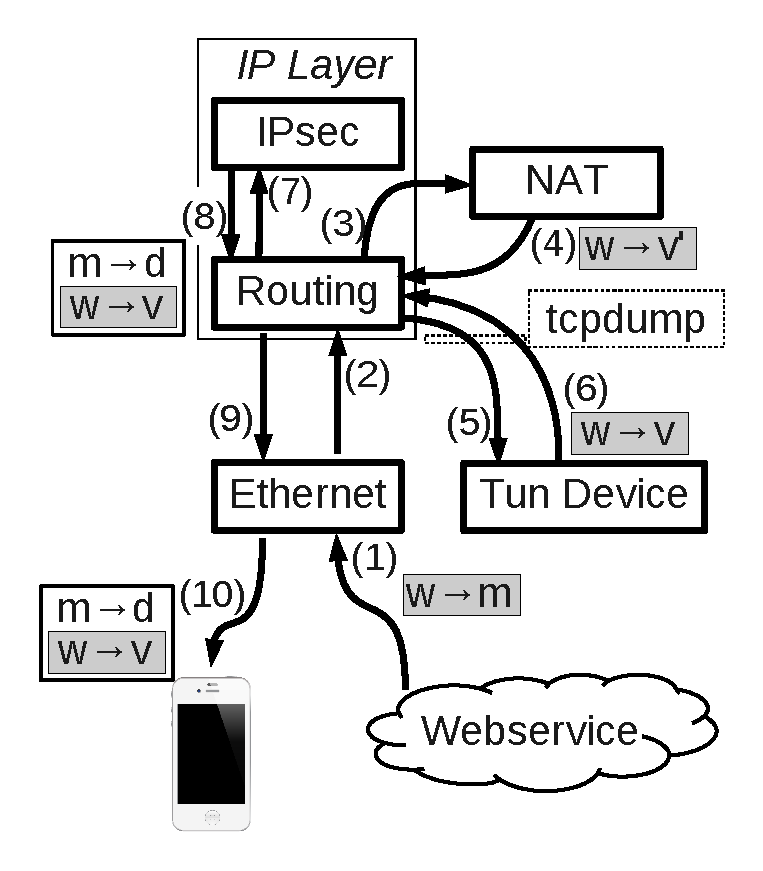
\includegraphics[width=0.47\columnwidth]{figures/packet-monitoring-d.pdf}}
\newline
\begin{small}
\begin{tabular}{|c|p{0.8\columnwidth}|}
\hline
Symbol & Description \tabularnewline
\hline
d & IP address of the mobile device assigned by its ISP. \tabularnewline
m & IP address of the \platname server. \tabularnewline
w & IP address of the server providing the Webservice. \tabularnewline
(i) & The i-th step of packet processing. \tabularnewline
\fbox{a $\rightarrow$ b} & Packet with source IP \emph{a} and destination IP \emph{b}. \tabularnewline
v & IP address of the mobile device in the VPN tunnel. \tabularnewline
v' & IP address of the mobile device while looping through tun device. \tabularnewline

\hline
\end{tabular}
\end{small}
\end{center}
\caption{Packet monitoring in the VPN proxy.}
\label{fig:packet-monitoring}
\end{figure}


An association between the mobile device and a packet is possible only if the packet encapsulated within an IPsec packets is monitored in the clear. 
However, the current implementation of NAT and IPsec makes this association of packets with the mobile devices non-trival.
A packet from the mobile device, encrypted using IPsec, needs to be decrypted before undergoing NAT. 
As shown in \fref{fig:packet-monitoring-problem}, because the IPsec computations take place after the NAT computations, the kernel loops the packet back to the IP layer after decryption.
This looping allows the packet monitor to observe the IPsec packet before and after decryption\footnote{A similar operation takes place if the mobile devices communicate with each other over P2P however we do not discuss this scenario due to lack of space.}.
When multiple flows pass through the VPN server, the packet monitor can use the private IP address to associate the packets with the mobile device. 
Once the NAT operation is performed the packet is forwarded via the network card.
When the network card receives a packet intended for the mobile device, as shown in \fref{fig:packet-monitoring-problem}, the packet first undergoes NAT followed by IPsec encryption. 
The encrypted packet is then sent to the mobile device. 
Because the packet is not looped through the packet monitor before encryption, the packet monitor is not able to see the packet after NAT and before encrpytion. 
This implies without any modifications, any off the shelf packet monitor shall fail to associate the packets destined for mobile devices with the corresponding mobile device. 

\begin{figure}
\begin{center}
\includegraphics[width=0.8\columnwidth]{figures/tun-device.pdf}
\end{center}
\caption{Tun-tap device to loop packets for packet monitoring.}
\label{fig:packet-monitoring-solution}
\end{figure}

To monitor the packets that are encapsulated within IPsec packets we route the packets through a tun-tap device before encryption and after decryption. 
As shown in \fref{fig:packet-monitoring-solution},

\subsubsection{Transparent Proxy}
\label{sec:platform-transparent-proxy}


\subsection{Feasibility}


\subsection{Caveats}


%%% Local Variables: 
%%% mode: latex
%%% TeX-master: "main.tex"
%%% End: 
